

\documentclass[11pt, oneside]{article}   	% use "amsart" instead of "article" for AMSLaTeX format
\usepackage{geometry}                		% See geometry.pdf to learn the layout options. There are lots.
\geometry{letterpaper}                   		% ... or a4paper or a5paper or ... 
%\geometry{landscape}                		% Activate for rotated page geometry
\usepackage[parfill]{parskip}    		% Activate to begin paragraphs with an empty line rather than an indent
\usepackage{graphicx}				% Use pdf, png, jpg, or eps§ with pdflatex; use eps in DVI mode
								% TeX will automatically convert eps --> pdf in pdflatex		
\usepackage{amssymb}
\usepackage{amsmath} 
\usepackage{bm}
\usepackage{xcolor}
\usepackage{bbm}
\usepackage{bbold}
\usepackage[T1]{fontenc}
\usepackage{subfigure}
\usepackage[english]{babel}
\newtheorem{theorem}{Theorem}[subsection]
\newtheorem{corollary}{Corollary}[theorem]
\newtheorem{lemma}[theorem]{Lemma}
\newtheorem{mydef}{Definition}

%SetFonts

%SetFonts


\title{Clicking Data}
\author{}
\date{}							% Activate to display a given date or no date

\begin{document}
\maketitle

\section{Simulation on time for full data}
\subsection{Simulation set up}
In this experiment, we want to compare the speed of the Mallows MCMC and the pseudolikelihood in inferring the consensus parameter $\bm{\rho}$. We first generate a dataset $\{\bm{R}^1, ..., \bm{R}^N \}$, i.e., a dataset that contains full ranking of $n$ items from all $N$ users by drawing i.i.d. samples from the Mallows distribution with a fixed $\bm{\rho}^0$ and $\alpha^0$. We then both use the Mallows MCMC and the pseudo-likelihood, with the known $\alpha^0$, to estimate $\bm{\rho}^0$. For each method, we run the algorithm multiple times, each run with a different number of iterations. For each run, we record the run time, compute the CP consensus of the samples, and then compute the foot rule distance between the CP estimation and $\bm{\rho}^0$. 

We try out different sets of parameters, and for each set of parameters, we generate 10 datasets. In Figure \ref{fig:full_time_simulation}, we plot the foot rule distance between the CP consensus and the true consensus / $n$ on the $y$ axis, and its corresponding run time on the x-axis. It can be observed that given enough time, the Mallows MCMC tends to give more correct estimation of the $\rho$ parameter, however, the pseudo-likelyhood is able to give reasonable estimations much faster. This is due to the fact that there is no burn-in period needed for the pseudo-likehood, and each sample is independently drawn, therefore, making the algorithm more efficient.

\textcolor{red}{Shoud I also show the time per iteration?}
\begin{figure}[hbt!]
	\begin{minipage}[t]{.32\linewidth}
		\centering
		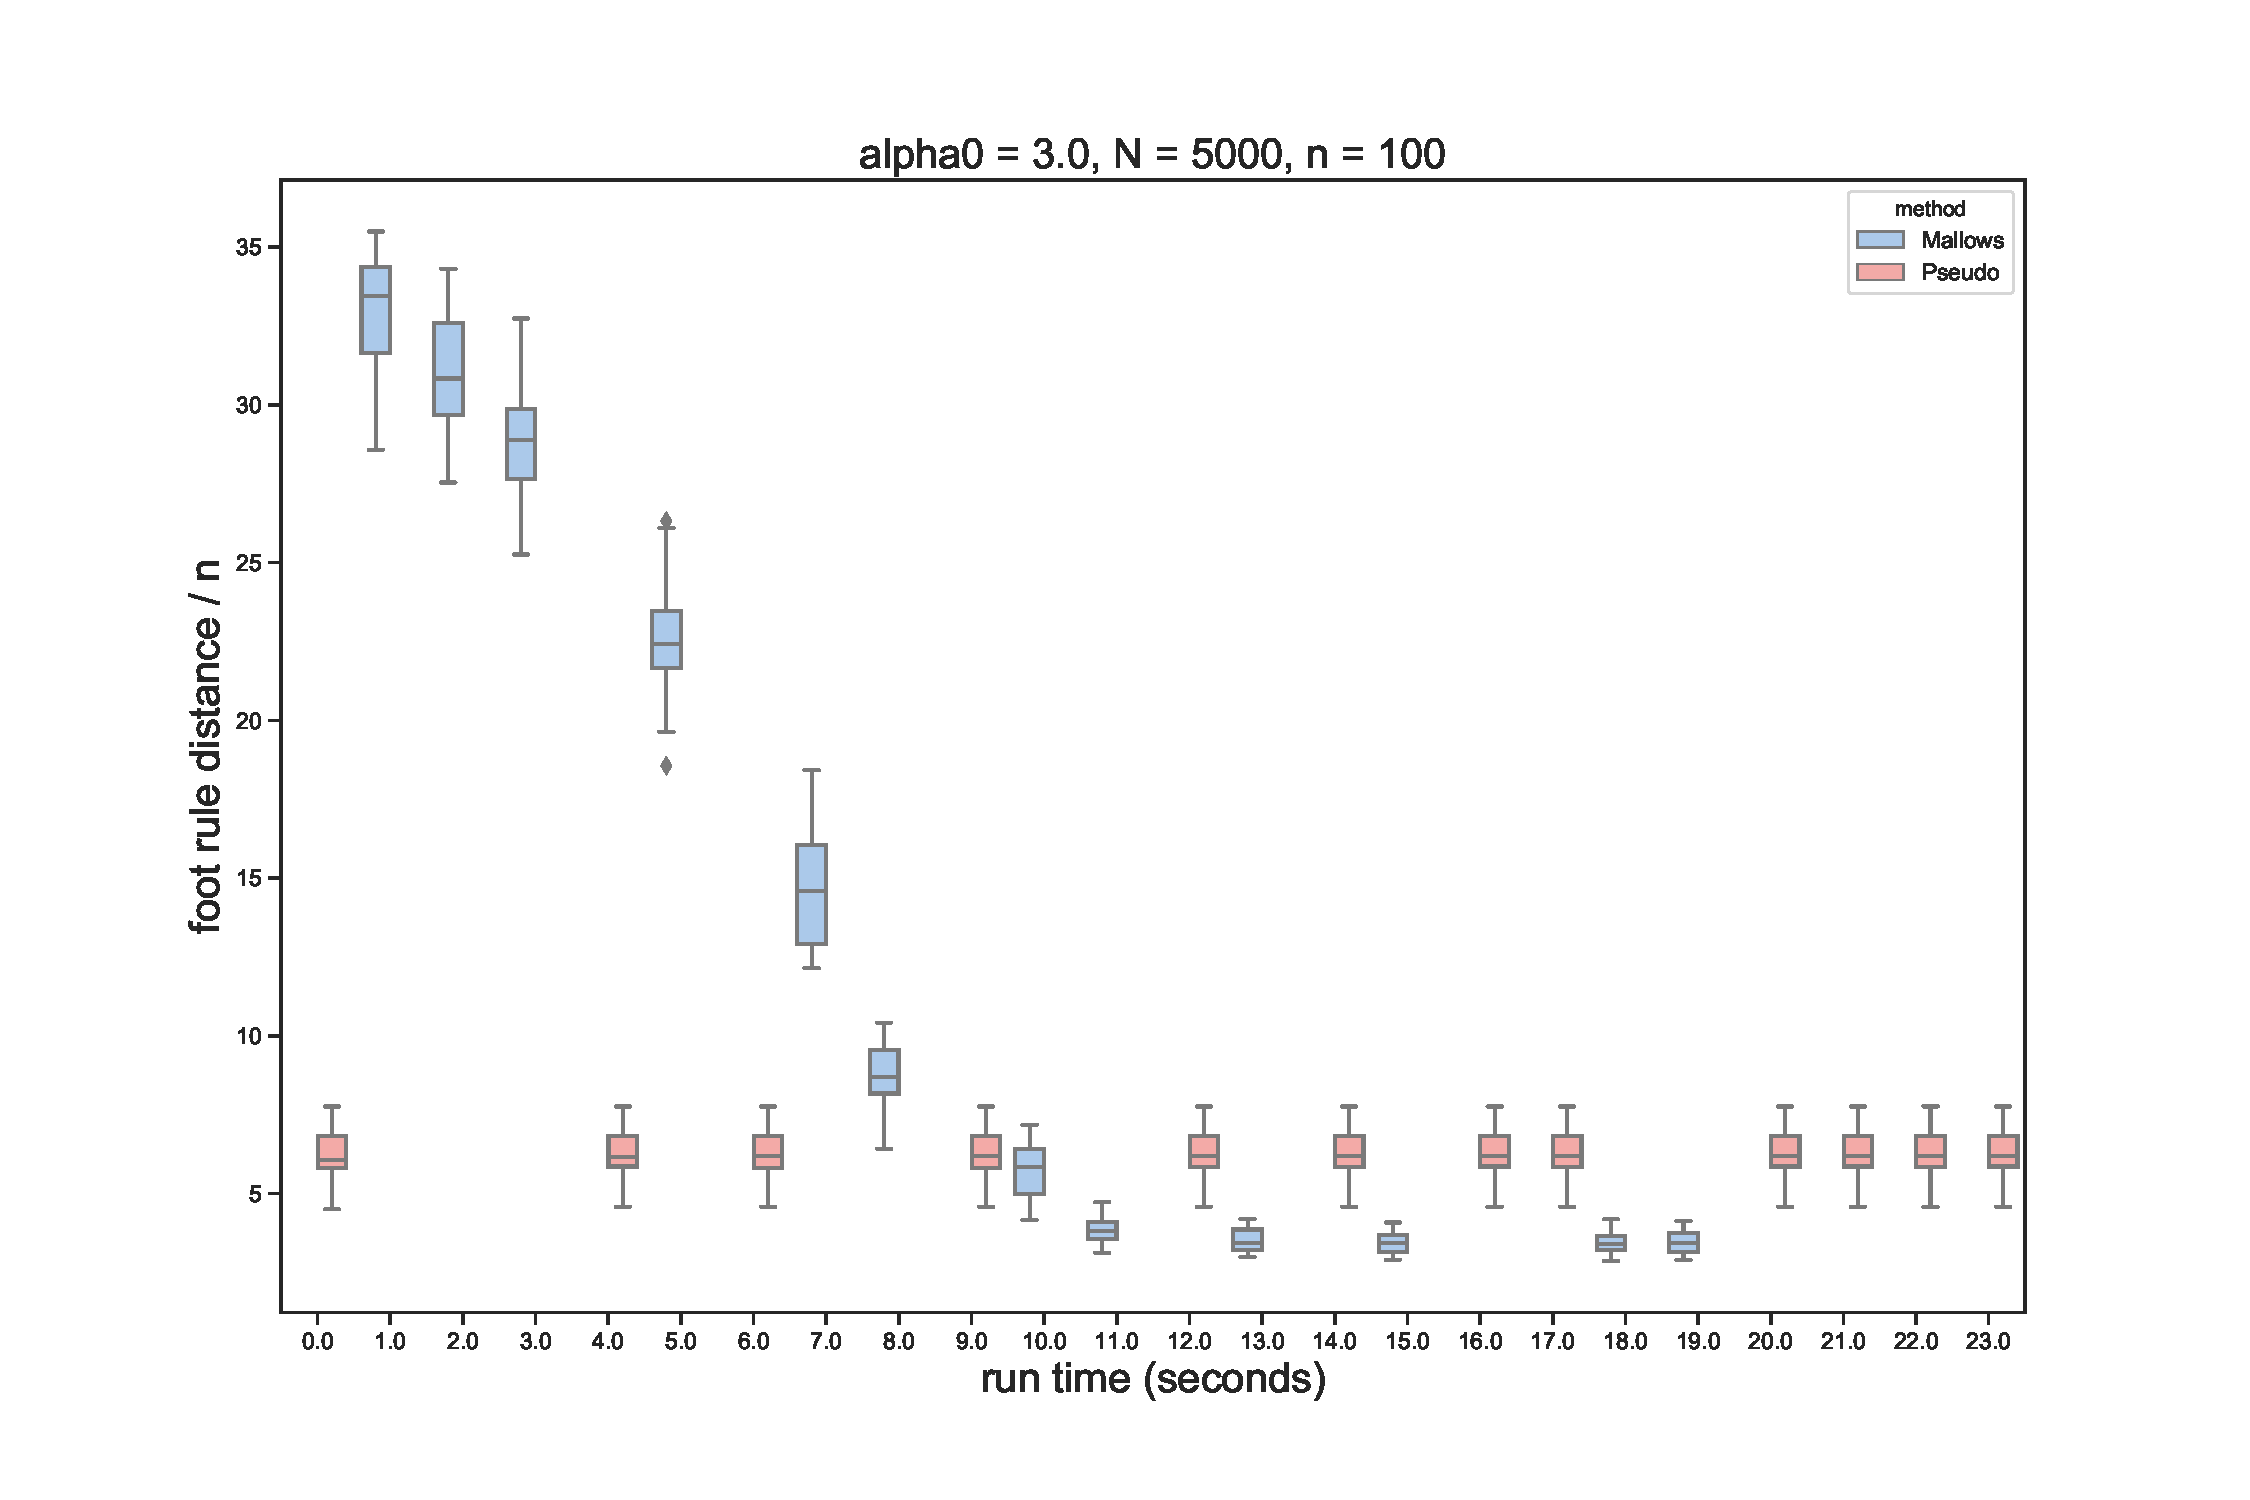
\includegraphics[width=\linewidth]{figures/full_time_simulation/box_alpha03N5000n100}
	\end{minipage}
	\begin{minipage}[t]{.32\linewidth}
		\centering
		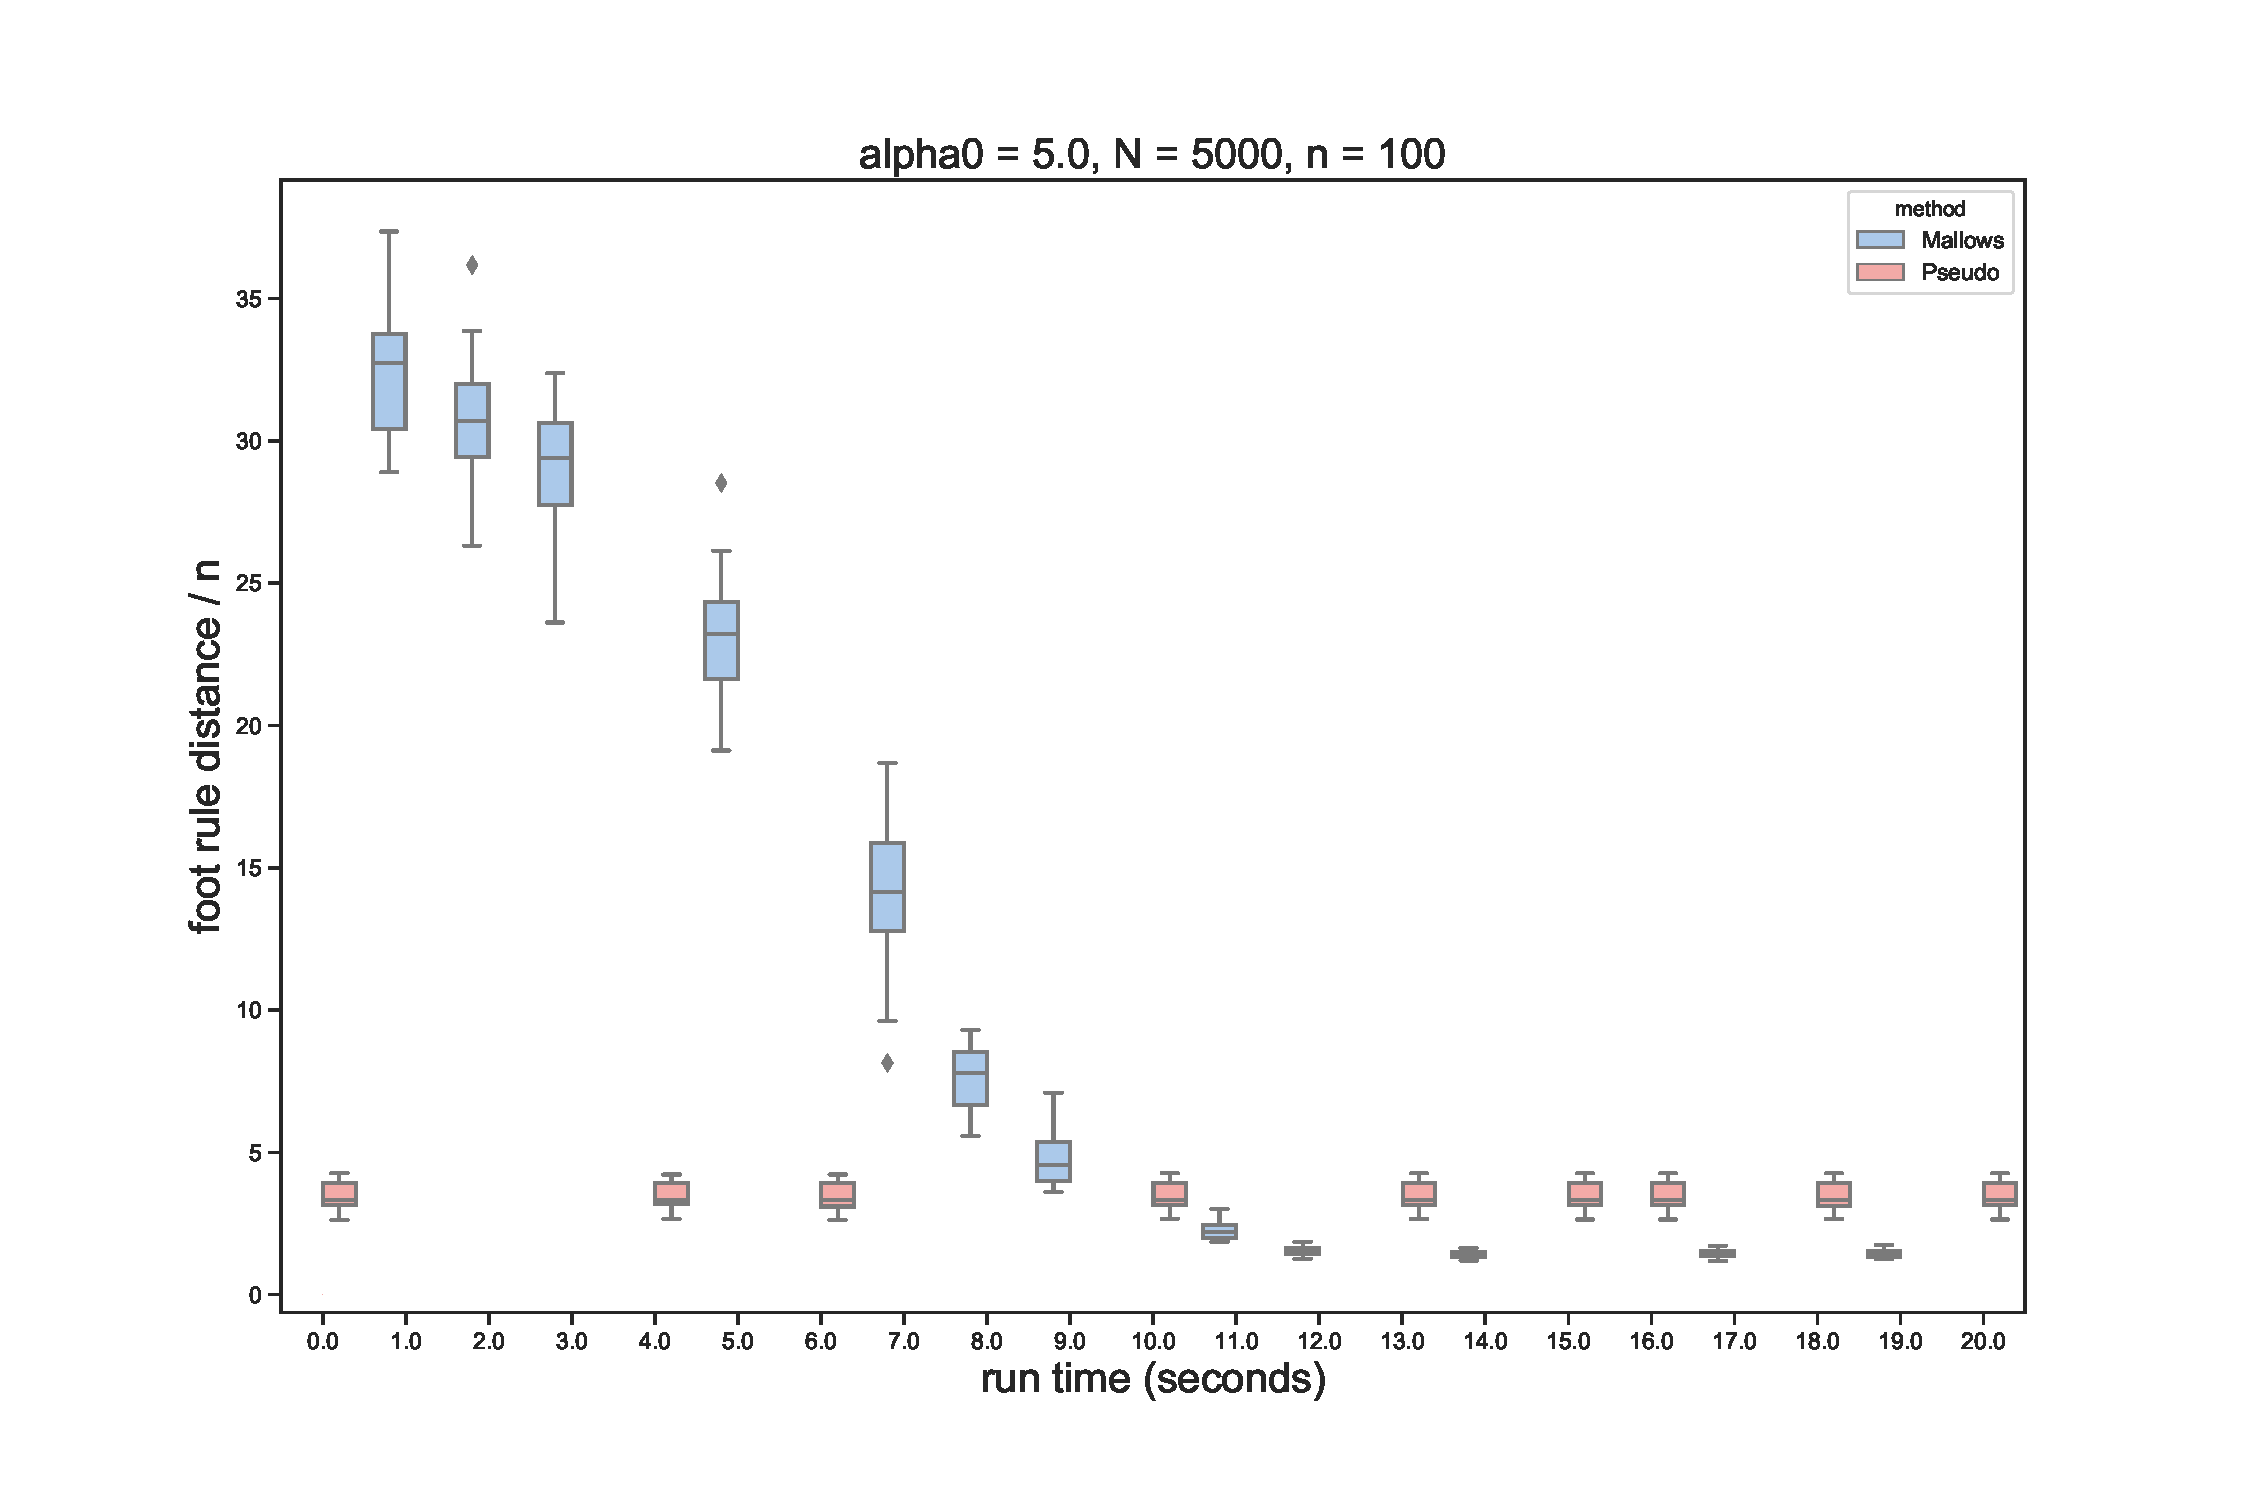
\includegraphics[width=\linewidth]{figures/full_time_simulation/box_alpha05N5000n100}
		
	\end{minipage} 
	\begin{minipage}[t]{.32\linewidth}
	\centering
	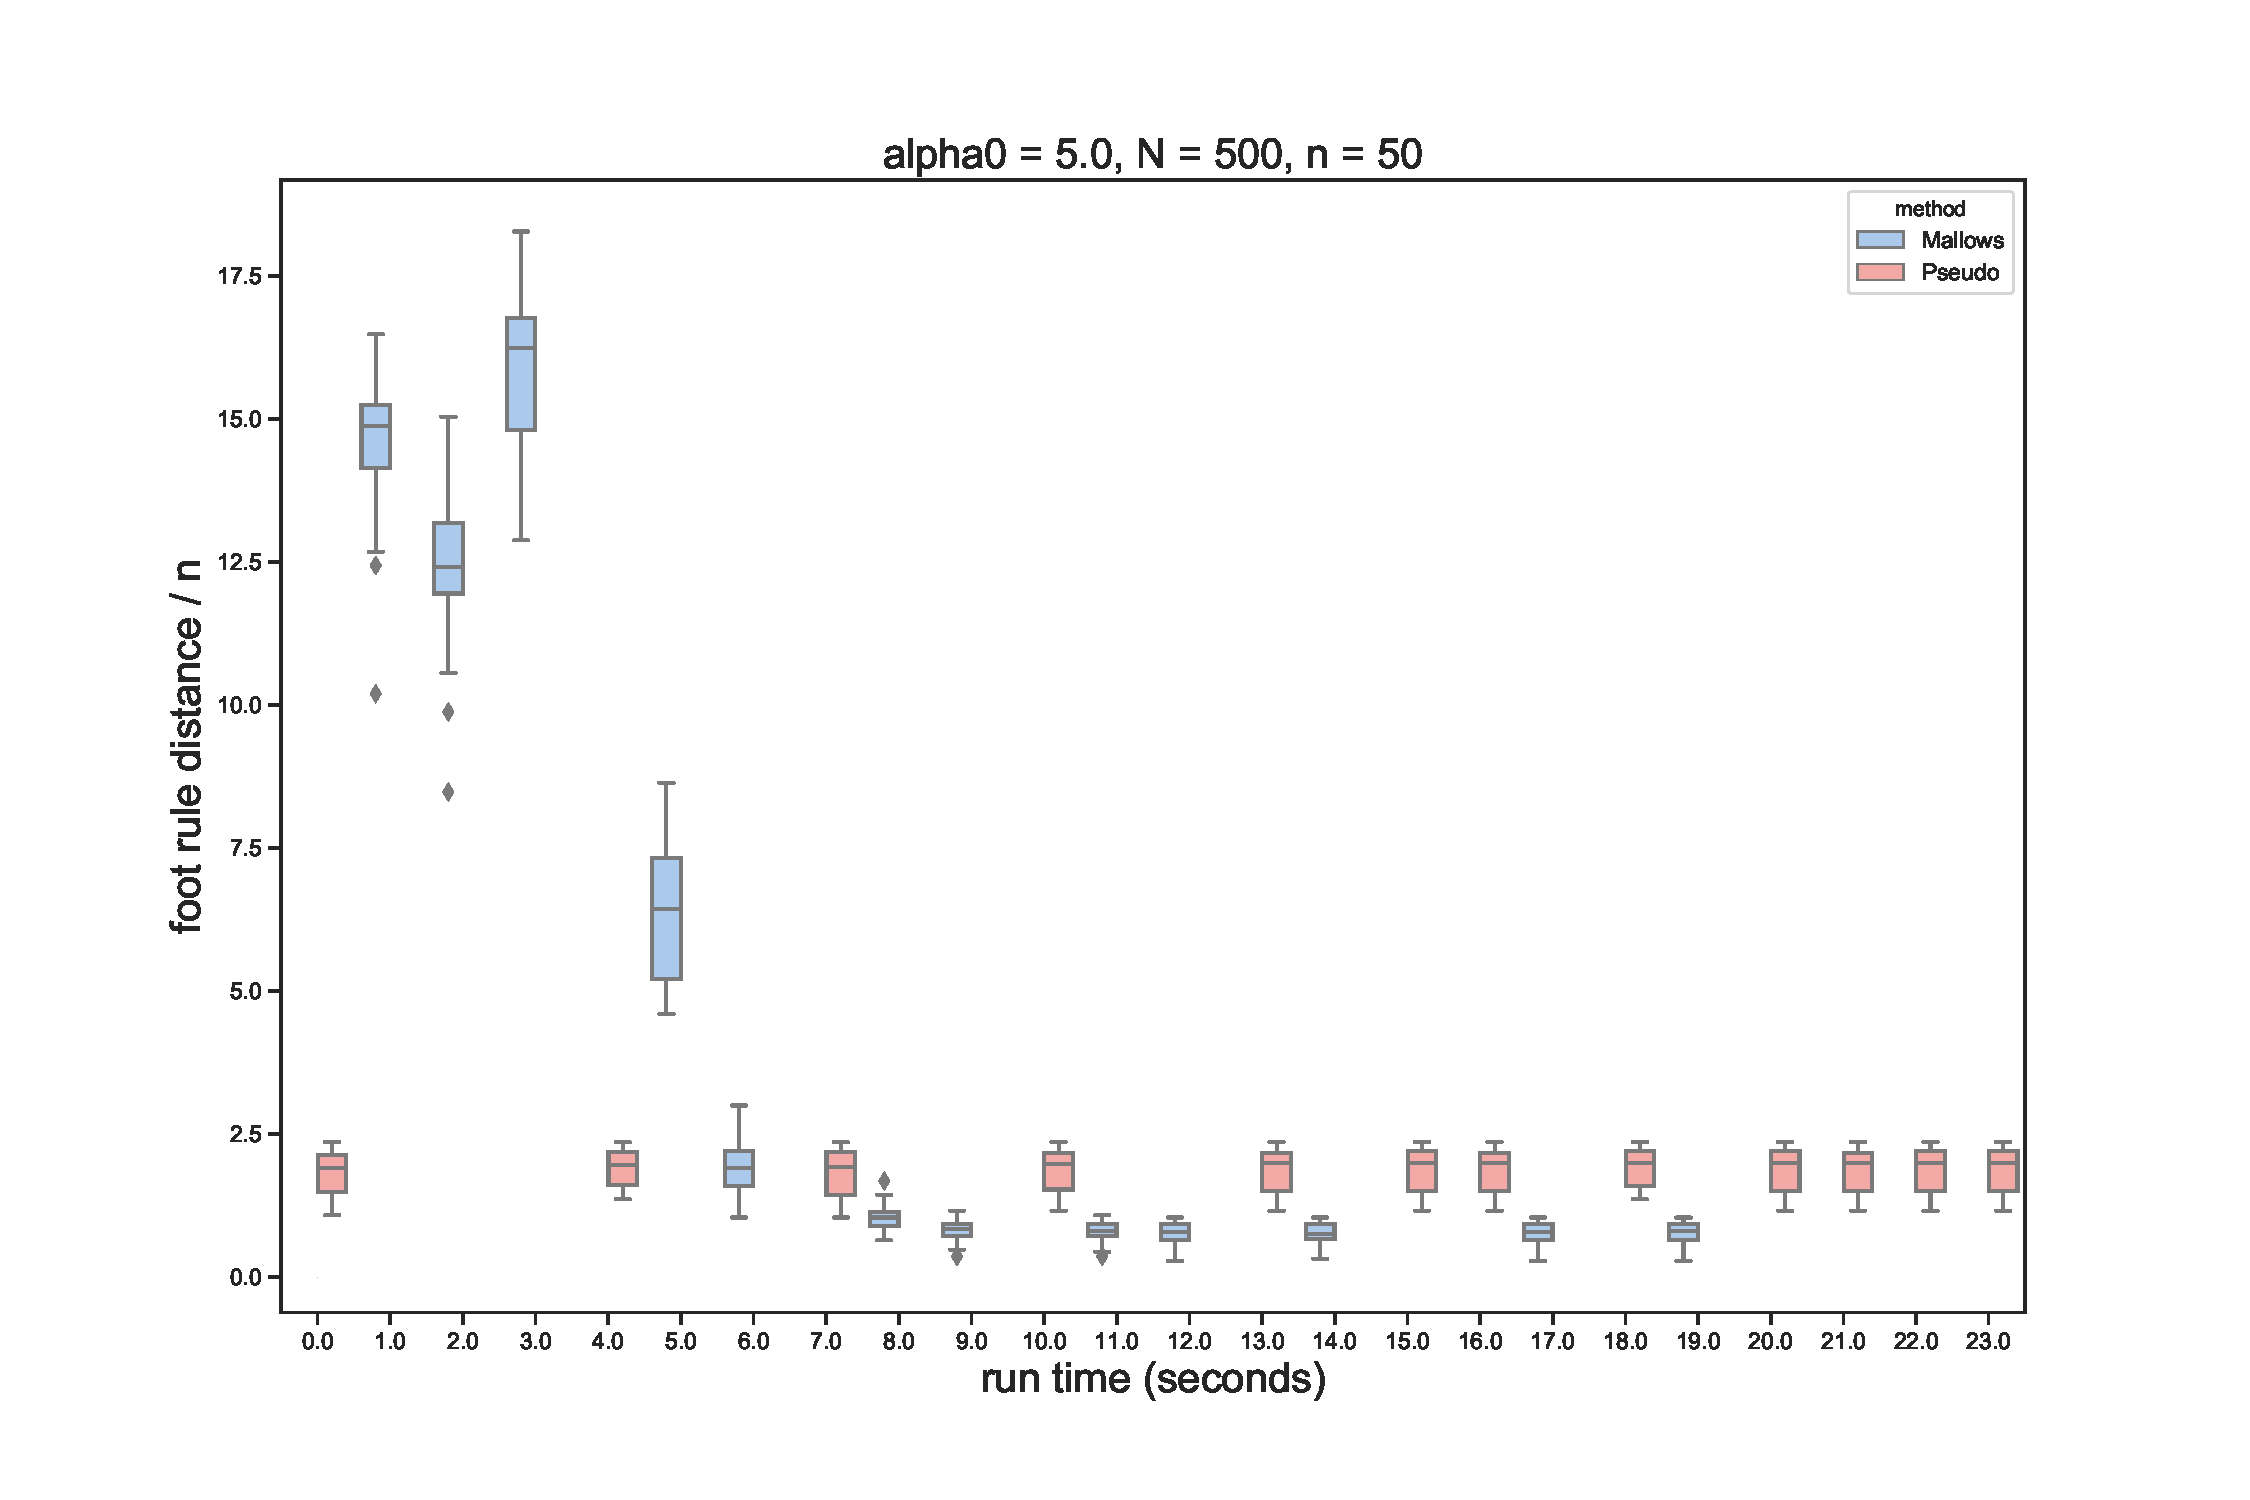
\includegraphics[width=\linewidth]{figures/full_time_simulation/box_alpha05N500n50}
	\end{minipage} 

	\caption{y-axis: d(CP consensus, $\bm{\rho}^0$)/$n$, x-axis: run time}
	\label{fig:full_time_simulation}
\end{figure}


\section{Simulation results - clicking data}
\subsection{General Notations}

\begin{itemize}
	
	\item {$c_j$: number of items clicked by user $j$}
	\item {$\mathcal{A}_j$: set of items clicked by user $j$, |$\mathcal{A}_j| = c_j$}
	\item {$\mathcal{A}_j^c$: set of items NOT clicked by user $j$, |$\mathcal{A}_j^c| = n-c_j$ }
	\item {$\bm{B}^j = \{b^j_1, ..., b^j_n\}$: a binary vector of length $n$, indicating user $j$'s clicks. $b^j_i$ = 1 if $i \in \mathcal{A}_j$, and 0 otherwise}
	
\end{itemize}
\subsection{Toy example set up}
In this section, we first simulate a dataset of $N = 20$ users, $n = 20$ items, $\bm{\rho}^0 = 1, ..., n$, and $\alpha^0 = 5$, by sampling from the Mallows distribution. The number of clicks for each user $c_j$ is drawn from a truncated poisson distribution, with a mean of 5 items, minimum of 1 item and maximum of 17 items. We recommend $ k = 2$ items for each user.  

\subsection{Comparison of $\bm{\rho}$}
A comparison of the distribution of $\bm{\rho}$ using the Mallows posterior and the pseudo-likelihood is shown on \textbf{Figure} \ref{fig:heat_rho}.
\begin{figure}[hbt!]
	\begin{minipage}[t]{.45\textwidth}
		\centering
		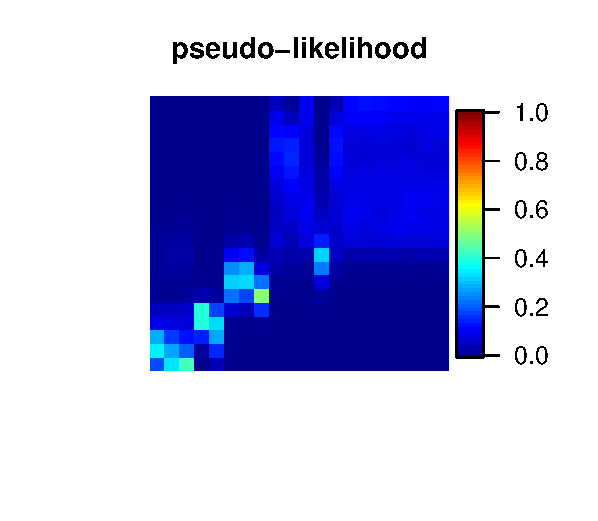
\includegraphics[width=\textwidth]{figures/clicking/Pseudo_rho_heat}
		
	\end{minipage}
	\hfill
	\begin{minipage}[t]{.45\textwidth}
		\centering
		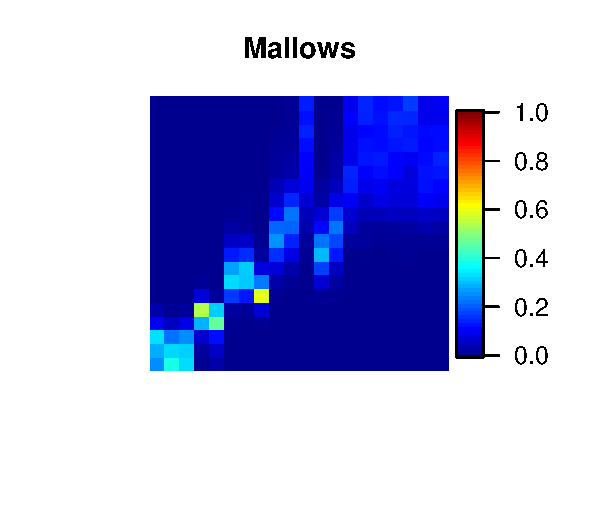
\includegraphics[width=\textwidth]{figures/clicking/Mallows_rho_heat}
		
	\end{minipage} 
	\caption{left: pseudo-likelihood, right: Mallows}
	\label{fig:heat_rho}
\end{figure}

\subsection{Heat plots of selected individual users}
Heat plots of 2 selected users are shown in \textbf{Figure} \ref{fig:heat_ind}. The distributions appear quite similar, except for a few items, in which using the pseudo-likelihood function produces a somewhat flatter distribution compared to using Mallows directly. 
\begin{figure}[hbt!]
	\begin{minipage}[t]{.45\textwidth}
		\centering
		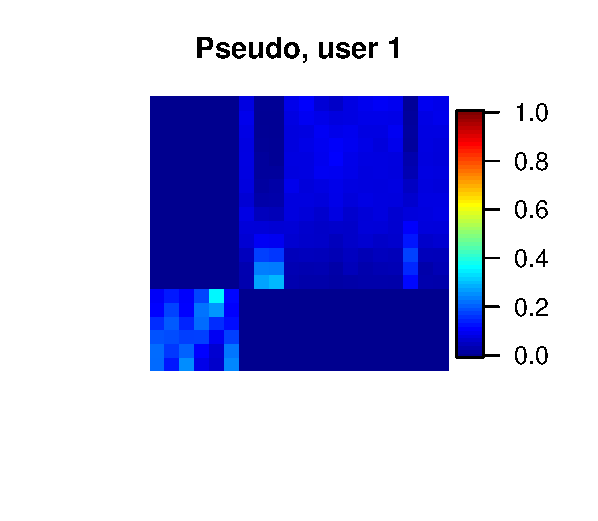
\includegraphics[width=\textwidth]{figures/clicking/pseudo_user1}
		
	\end{minipage}
	\hfill
	\begin{minipage}[t]{.45\textwidth}
		\centering
		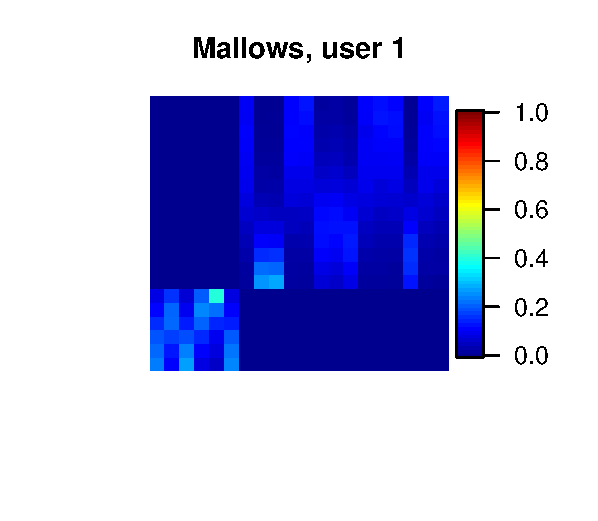
\includegraphics[width=\textwidth]{figures/clicking/mallows_user1}
		
	\end{minipage} 
	\begin{minipage}[t]{.45\textwidth}
	\centering
	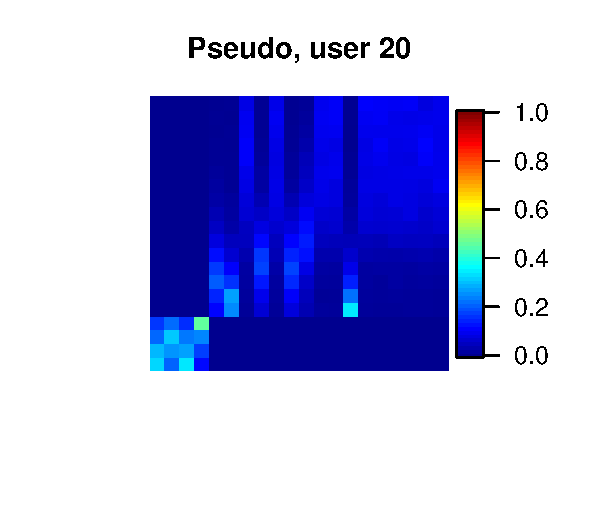
\includegraphics[width=\textwidth]{figures/clicking/pseudo_user20}
	
	\end{minipage}
	\hfill
	\begin{minipage}[t]{.45\textwidth}
		\centering
		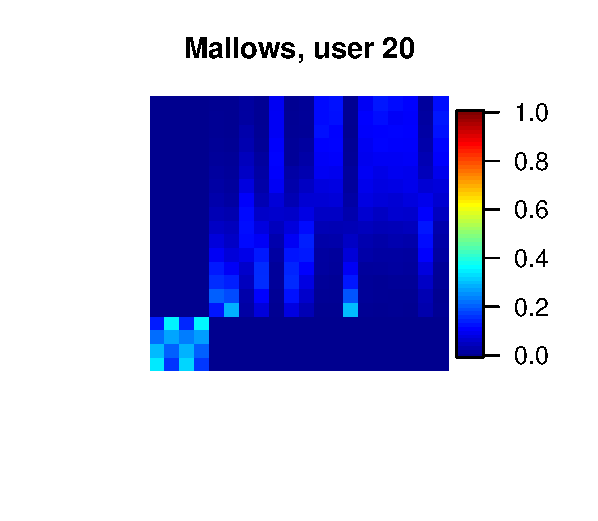
\includegraphics[width=\textwidth]{figures/clicking/mallows_user20}
		
	\end{minipage} 

	\caption{left: pseudo-likelihood, right: Mallows. The items are sorted according to the truth of the individual}
	\label{fig:heat_ind}
\end{figure}

\subsection{Recommendation accuracy}
In this particular toy example, the Pseudolikelihood 45\% of items are correctly recommended, while Mallows performs slightly better at 50\%.
\subsection{Special notes}
No Gaussian variation is introduced at this stage for the pseudo-likelihood; i.e., $\sigma = 0$. For each user $j$, the sequence for which items are to be sampled are based on a uniform distribution. (The V-ordering is tried out but don't seem to improve recommendation accuracy here). The $\alpha^0$ used for sampling is set at 10, instead of its real value 5. But the different choices of $\alpha^0$ don't seem to affect the resulted heat plots much.

\end{document}  